\section{Introduction}
\label{sec:introducntion}
In biological research, multiple sequence alignment (MSA) is a useful and/or essential task in various applications such as phylogeny estimation, prediction of the structure and function of a RNA or protein, identification of functionally important sites, orthologous gene identification etc. The MSA task seeks to arrange more than two biological sequences to infer homology, based on certain criteria such as evolutionary history, 3D structure etc. The output is a matrix in which the input sequences are the rows and each column (i.e., site) has letters (i.e., nucleotides or amino acids) which are homologous which means all those letters descend from the same letter of a common ancestor). The aligned sequences reflect historical substitution, insertion and deletion of genetic materials which are represented as gaps. Accurately recovering these properties through MSA is necessary to accomplish a biological objective such as inferring the evolutionary history relating the sequences known as phylogenetic trees. While computing MSAs, various computational methods and criteria are used to make hypotheses about homology. But the goal of MSA is entirely biological. Figure~\ref{fig:msa_io} illustrates this problem using a hypothetical example where four protein sequences of varying lengths need to be simultaneously aligned by inserting ``appropriate'' gaps to identify homology. In this research, we limit our focus on MSA in the context of phylogeny. Phylogeny estimation from molecular sequences generally operates as a two-phase approach. At first the given sequences are aligned using an MSA method, and then a tree is estimated from the resultant alignment. The quality of inferred trees heavily depends on the quality of the corresponding alignment. There is a large body of literature in the biological domain about the relationships between multiple sequence alignments and phylogenetic trees which laid the background for this study. For example, we find several studies~\cite{jordan2011effects, chang2014tcs, lake1991order, croan1997evolution, ogden2006multiple, wu2012accounting} analyzing the effects of alignment errors and uncertainty on the accuracy of phylogenetic tree reconstruction. Therefore, it is important to select an MSA tool that is the ``most suitable'' in the phylogenetic context.

\begin{figure}[!htbp]
	%\centering
	\begin{adjustwidth}{-0.2cm}{-0.2cm}
		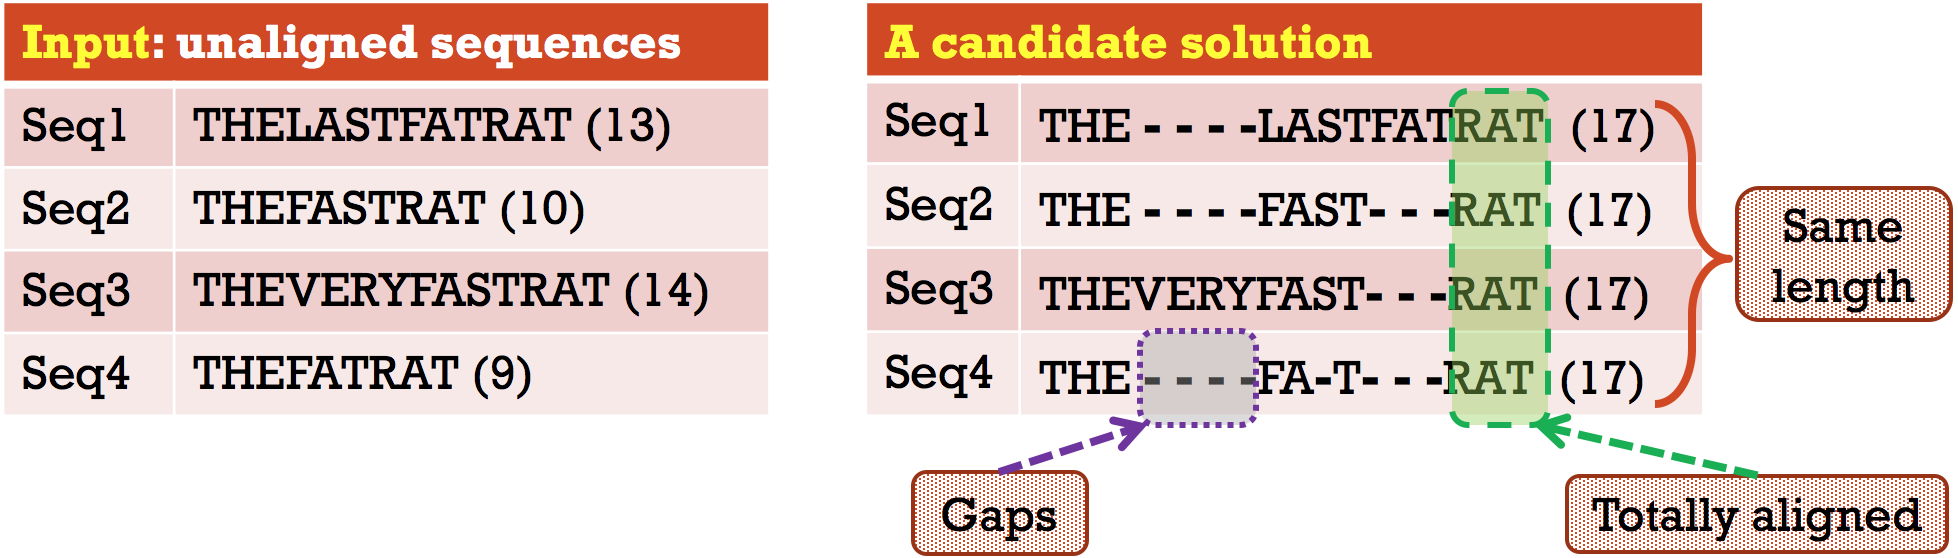
\includegraphics[width=0.5\textwidth]{Figure/msa_io}
		%\vspace{-0.6cm}
		\caption{A hypothetical example of an MSA problem.} 
		\label{fig:msa_io}
	\end{adjustwidth}
\end{figure}

In this study, we aim to design a multi-objective formulation of MSA that is more effective in phylogeny estimation. Previously several researchers (\citep{redelings2005joint, ashkenazy2018multiple}) made an attempt to improve the phylogeny estimation focusing on MSA computation. While they also agree with our core idea that the nature of MSA computation may influence the outputs (in a domain specific manner), they do not focus on any application-aware multi-objective formulation. %worked on the same core idea and provided solid proof of concept. We differ from them by adopting the multi-objective approach.
Our motivation for a multi-objective formulation comes from the fact that the alignment estimated under one objective may be different to the alignments generated under other objectives, inferring discordant homologies and thus leading to different and often conflicting evolutionary histories relating the sequences under consideration. Multi-objective formulations can address this issue by optimizing multiple conflicting objectives simultaneously to generate a set of alignments. However, we are faced with the challenge of using appropriate measures/metrics to choose from among a number of objective sets to optimize. So, we ask the natural question whether the popular general purpose measures to judge the alignment quality can truly reflect the quality in the context of a particular application domain, i.e., phylogeny estimation in our case. While this question has received some shallow discussion in several studies (\citep{warnow2013large, mirarab2015pasta, liu2009rapid}), to the best of our knowledge no systematic investigation has been reported in the literature to this end. Therefore, in essence, we systematically investigate whether an application-aware metric can guide us better in choosing appropriate multi-objective formulation or tools capable of generating alignments that can produce better phylogenetic trees.


There are numerous tools available in the literature to compute MSAs. We can broadly divide them into three groups: progressive techniques, consistency based techniques and iterative techniques. This division is not exclusive as many tools also use a combination of these techniques. Progressive technique is the foundation of many MSA tools such as, Clustal $\Omega$~\citep{sievers2011fast}, PRANK~\citep{loytynoja2005algorithm}, Kalign~\citep{lassmann2008kalign2}, FSA~\citep{bradley2009fast}, RetAlign~\citep{szabo2010reticular} etc. They compute the alignment using a guide tree by aligning pairs of sequences in a ``bottom-up'' manner. Among them, FSA employs an explicit statistical model to generate the alignments. It is the only method that gives an estimation of uncertainty for every column and character of the alignment. Moreover, it utilizes machine-learning techniques to estimate gap and substitution parameters at runtime for each input data. 

The consistency based techniques first construct a database of local and global pairwise alignments to facilitate generating an overall accurate alignment. The representatives of this category are T-Coffee~\citep{notredame2000t}, ProbCons~\citep{do2005probcons}, MSAProb~\citep{liu2010msaprobs}, ProbAlign~\citep{roshan2006probalign} etc. On the other hand, the iterative techniques were designed to achieve reliable alignments. These techniques try to fix the effect of mistakes made during the initial phases by repeating some crucial steps until some criteria are met. We find several examples of such techniques, such as, MAFFT~\citep{katoh2002mafft}, MUSCLE~\citep{edgar2004muscle}, MUMMALS~\citep{pei2006mummals}, ProbCons%, PRIME~\citep{yamada2006improvement}, SAGA~\citep{notredame1996saga} 
etc. In this category, we also see some ``meta-methods'' such as, SAT\'e~\citep{liu2009rapid} and PASTA~\citep{mirarab2015pasta}, which co-estimate alignment and tree using other methods. These tools achieve scalability by employing the divide-and-conquer principle and are being used widely in practice.

The performance of an MSA tool is usually evaluated by comparing its output alignment with the reference alignment (provided with the dataset as the ground truth) in terms of several measures. To this end, the most popular measures are perhaps sum-of-pair (SP) score and total-column (TC) score. SP score is the fraction of the homologies (i.e., pairs of aligned characters) in the reference alignments recovered in the estimated alignment. Similarly, TC score is the fraction of the actual aligned columns that appear in the estimated alignment.
%; both of these measures are well-known basics in MSA literature and will be defined shortly in a subsequent section. 

In this post-genomic era, the MSA datasets are posing new challenges to the researchers. Usually, an MSA method is provided with a default parameter configuration for aligning any problem instance with satisfactory accuracy. But we know that these default values can not guarantee the best output throughout all kinds of datasets~\citep{rubio2018characteristic}. For instance, there is a parameter in ProbCons called the number of iterative refinement passes. Although it can vary between 0 to 1000 the default value is set to 100. We can achieve better results by tuning the parameter values which is not a straightforward task. A systematic approach, namely, parameter advertising~\citep{deblasio2015parameter}, helps to choose the best parameter setting of an MSA method for each input data. Moreover, despite rigorous parameter tuning, no method can consistently outperform other methods for all datasets. 

Therefore, we see the emergence of novel approaches that combine different alignment tools \citep{thompson2011comprehensive}. One such approach is metaheuristics where alignments generated from different tools are exploited to produce improved alignments without vesting any effort in parameter tuning. The success of such a metaheuristic approach depends on the selection of proper objective function that can help to select better solutions from among the alternatives and thereby guide the search process towards optimal solutions of MSA.
%can push the solutions (i.e., alignments) towards the desired zone that reflects the actual purpose of an alignment task. 
As any single objective function alone can not be effective to tackle different challenges, it is wise to simultaneously optimize multiple objective functions. This will produce a set of competing solutions as the final output, which can be expected to contain our desired solution(s). Thus the formulation of MSA as a multi-objective optimization problem turns out to be appealing.

During the last decade, we find several studies (\citep{da2010alineaga, ortuno2013optimizing, soto2014multi, abbasi2015local, rubio2016hybrid,zambrano2017comparing}) with multi-objective formulation for MSA have been published -- proposing two to four objective functions to capture and quantify different aspects of an alignment. Among them, probably the most popular is the sum-of-pairs score and its weighted variants, where pairwise score is calculated for each pair of aligned sequences using a substitution matrix. This matrix should reflect the characteristics of the data at hand. Although we know that the same character across all rows of a column does not necessarily indicate homology, the count of such columns in an alignment is seen as a maximization objective known as totally conserved columns. Next, we find attempts to minimize total number of gaps to maintain the compactness of an alignment. Then there are different types of gap penalties that penalize each sequence for introducing gaps. Also we find two other objective functions, Entropy and Similarity, that compute column-wise scores and then sum those together. Both of them try to express the homogeneity of characters in a column using two different ways. Contrary to the performance/quality measures mentioned earlier (such as SP score, TC score), we are not allowed to use the reference alignment while calculating these objective functions. 

We notice several \commentA{issues} in the works advocating multi-objective formulation of MSA (in the context of different applications where the MSA will be used). First of all, in these works, there is a lack of sound theoretical or empirical justification for the choice of a particular objective function to be optimized. Secondly, we also notice the absence of a sound rationale/justification behind the two most popular performance metrics, namely, sum-of-pair score and total column score. On the contrary, it seems only natural that performance score should reflect the actual purpose of MSA. For example, if the goal is to estimate a phylogenetic tree, the performance metric to be used for evaluation should be able to accurately measure the quality and usefulness of the constructed tree. Notably, another \commentA{issue}, specific to the domain of phylogeny estimation, is the use of relatively smaller (number of taxa below 50) datasets in experiments. 
%Moreover, those works used relatively smaller datasets with number of taxa being less than 50. 

In this article, we attempt to demonstrate the effectiveness of multi-objective MSA by addressing the above mentioned limitations in the context of its intended application domain (i.e., phylogeny estimation).
%We choose a multi-objective formulation from existing studies based on their potential to produce good phylogenetic trees. Afterwards, we propose a new formulation following a similar trend. 
To make a fair comparison with nine state-of-the-art MSA tools, we conduct comprehensive experimentations on both simulated and biological datasets using tree as well as alignment quality measures. 
%We make our source code public at~\url{https://github.com/ali-nayeem/MSA}. 
Our study represents the only known work on devising a phylogeny-aware multi-objective formulation for MSA. In particular, this article makes the following key contributions:
\begin{itemize}
	\item To the best of our knowledge, this is the first attempt to investigate whether a domain specific measure (as opposed to generic alignment measures) can guide us better in choosing an appropriate multi-objective formulation or tool for MSA when the goal is to infer phylogeny. Notably, although there exist some prior works that proposed different approaches in MSA computation (such as averaging MSA~\citep{ashkenazy2018multiple}) to improve phylogeny reconstruction, our novelty lies in providing an application-aware multi-objective formulation for MSA.
	
	\item We suggested a methodology based on multiple linear regression to judge the potential efficacy of a multi-objective formulation of MSA. Then, based on this methodology, we proposed two multi-objective formulations that had the potential to yield better phylogenetic trees.
	
	\item Finally, we demonstrated that the multi-objective formulations can consistently yield better phylogenetic trees than several state-of-the-art MSA tools. Following our methodology, we identified \{SimG, SimNG\} to be the best set of objective functions for computing MSAs with an aim to infer phylogeny, considering its overall accuracy, runtime and nonparametric nature. And, interestingly we found that popular alignment quality measures do not necessarily lead to highly accurate phylogenetic trees. 
	
	\comment{ 
		\item \underline{Here starts the old contributions:} \\We first studied a phylogeny-aware multi-objective MSA formulation by examining how an objective function associates with the phylogenetic tree quality.
		\item We demonstrated that, the multi-objective optimization of MSA can consistently outperform several state-of-the-art MSA tools.
		\item We conducted a series of statistical tests to establish the significance of differences between the performance (with respect to phylogenetic tree) of multi-objective formulation and the MSA tools.
		\item We empirically show that, optimizing widely used alignment quality measures may not lead us to better phylogenetic trees.
		\item Our study revealed two simple and non-parametric (which does not depend on the characteristics of the dataset) objective functions which are effective for phylogeny estimation. 
	}
\end{itemize}
 